\section{New Data}
\subsection{General Information}
\begin{frame}{General information}
\small
\begin{minipage}[c]{0.55\textwidth}
  \begin{itemize}
    \item to be certain in our droplet measurements we normally compare gas-jet and droplet experiments
    \item \textbf{Gas-jet}: free rotating molecule at around \textbf{10-15K}
    \item \textbf{Droplets}: molecules attach \textbf{helium belt} and are cooled down to about \textbf{0.4K}
  \end{itemize}
\end{minipage}\hfill
\begin{minipage}[c]{0.05\textwidth}
  \centering
  \scalebox{2.5}{$\Rightarrow$}
\end{minipage}\hfill
\begin{minipage}[c]{0.40\textwidth}
  \small
  \begin{itemize}
    \item different \textbf{B} and \textbf{D} rotational constants
    \item different thermal \textbf{state} distribution
    \item \textbf{interactions} with the helium in droplets 
  \end{itemize}
\end{minipage}
\linebreak
\linebreak
\linebreak
Typical model used to describe the molecule state: \textbf{Rigid Rotor with Centrifugal Distortion}
\begin{equation*}
      E(J) =  BJ(J+1) - DJ^2(J+1)^2
\end{equation*}
\begin{minipage}[c]{0.60\textwidth}
  \centering
  $\rightarrow$ the \textbf{wall} !!!
\end{minipage}\hfill
\begin{minipage}[c]{0.40\textwidth}
  \centering
  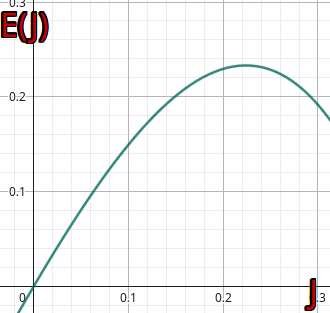
\includegraphics[width=.4\linewidth]{pic/wall.png}
\end{minipage}
\end{frame}

\begin{frame}{Energy dissipation in superfluid helium}
\textbf{Landau velocity} (ideal picture)
\begin{itemize}
  \item  no energy dissipation/ elementary excitation in the superfluid below critical kinetic energy
  \item "friction" through excitation of Rotons
\end{itemize}
\small
\begin{minipage}[c]{0.60\textwidth}
  \centering
  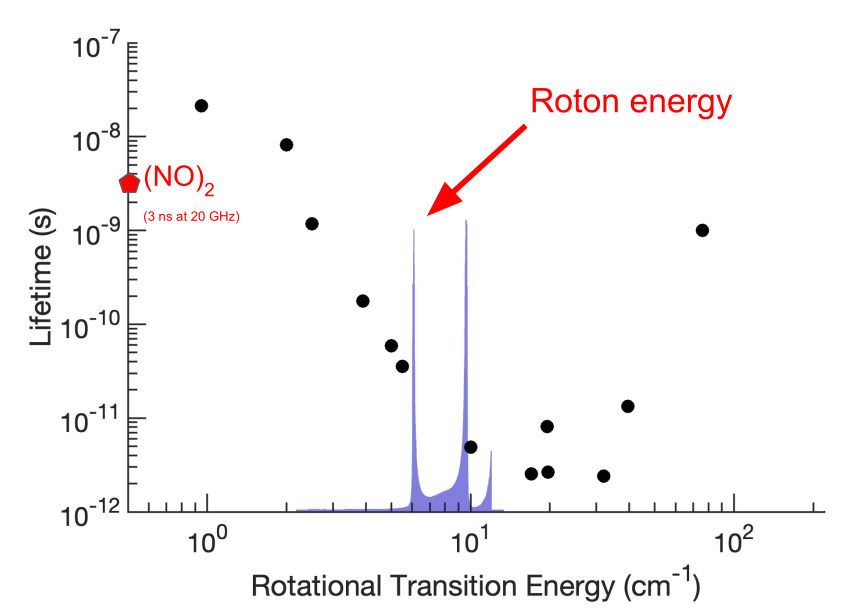
\includegraphics[width=.8\linewidth]{pic/roton_dos.png}
\end{minipage}\hfill
\begin{minipage}[c]{0.40\textwidth}
  \small
  \begin{itemize}
    \item only experimentally determined lifetimes
    \item different measurement methods
    \item Roton energy around \textbf{180 GHz}
  \end{itemize}
\end{minipage}
\end{frame}
\subsection{CS2 in Droplets}
\begin{frame}{CS2 - fast centrifuge}
  \begin{minipage}[c]{0.7\textwidth}
  \centering
  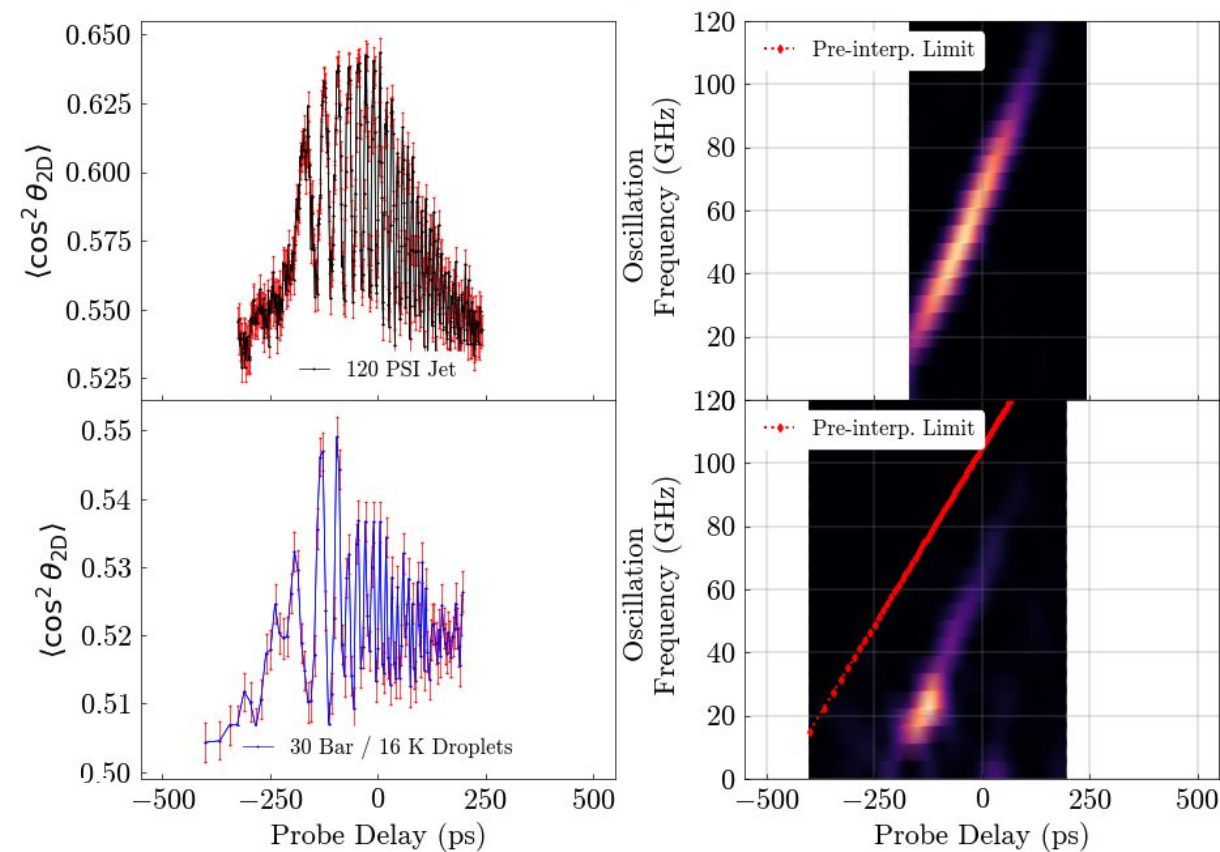
\includegraphics[width=.9\linewidth]{pic/cs2.png}
  \end{minipage}\hfill
  \begin{minipage}[c]{0.30\textwidth}
    \small
    \begin{itemize}
      \item wall at \textbf{20 GHz}
    \end{itemize}
    \vskip 20pt
    \textbf{New:}
    \begin{itemize}
      \item break through wall
      \item intensity decrease
    \end{itemize}
\end{minipage}
\end{frame}

\subsection{OCS in Droplets}
\begin{frame}{OCS - slower centrifuge}
  \begin{minipage}[c]{0.7\textwidth}
  \centering
  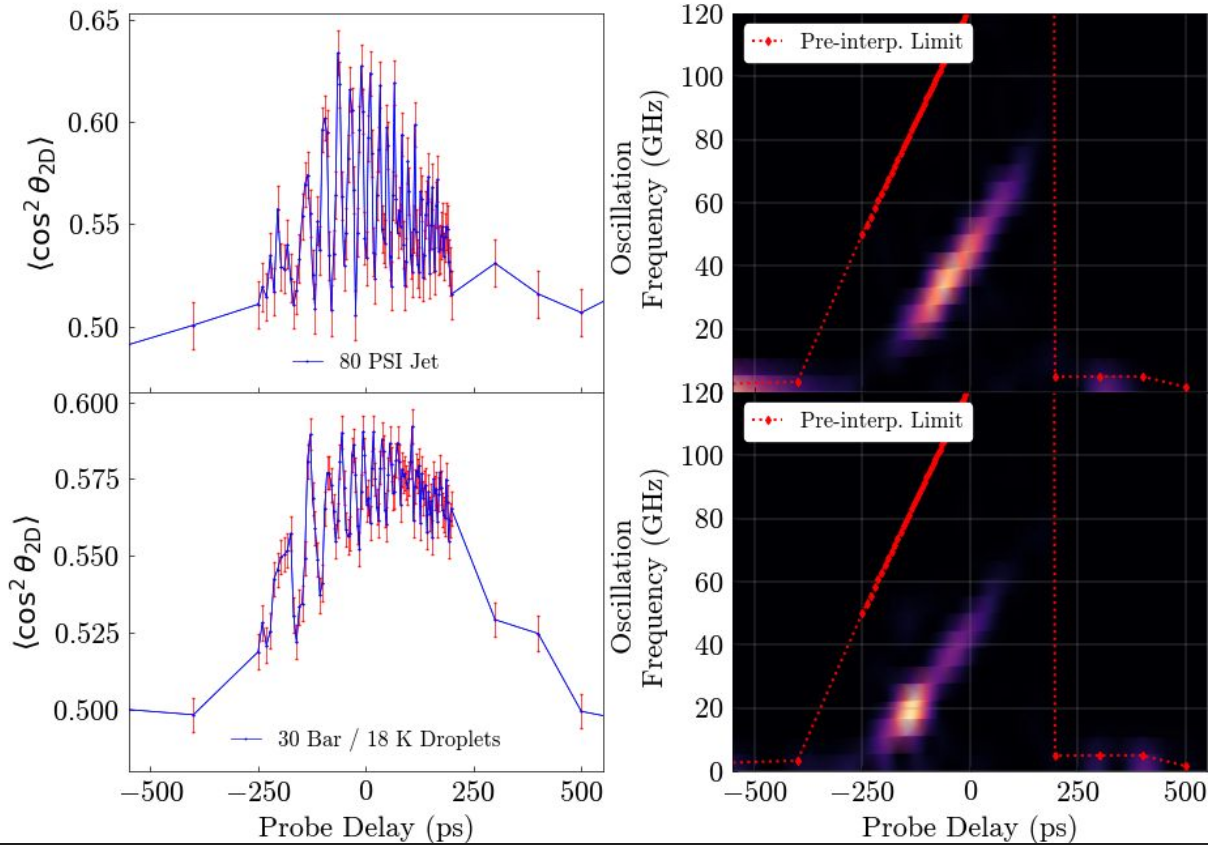
\includegraphics[width=.9\linewidth]{pic/ocs.png}
  \end{minipage}\hfill
  \begin{minipage}[c]{0.30\textwidth}
    \small
    \begin{itemize}
      \item wall at \textbf{38 GHz}
    \end{itemize}
    \vskip 20pt
    \textbf{New:}
    \begin{itemize}
      \item decrease in intensity at around the same frequency
      \item higher baseline
    \end{itemize}
\end{minipage}
\end{frame}

\begin{frame}{Modelling the in-field dynamics}
  \begin{minipage}[c]{0.7\textwidth}
  \centering
  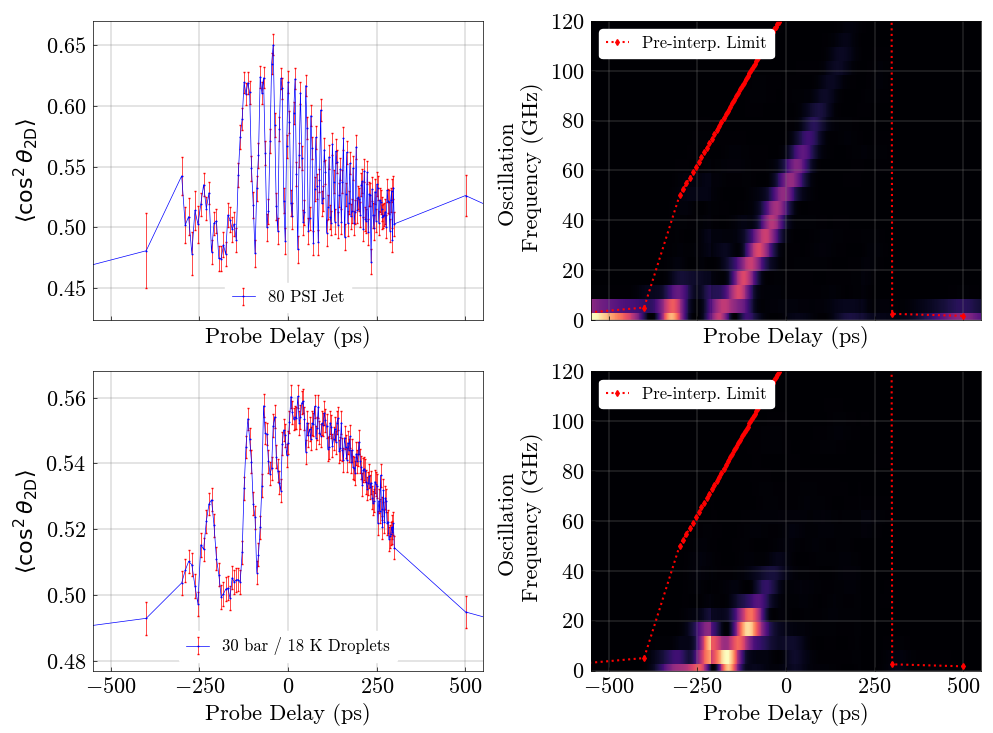
\includegraphics[width=.9\linewidth]{pic/ocs_fast.png}
  \end{minipage}\hfill
  \begin{minipage}[c]{0.30\textwidth}
    \small
    \begin{itemize}
      \item wall at \textbf{38 GHz}
    \end{itemize}
    \vskip 20pt
    \textbf{New:}
    \begin{itemize}
      \item not following after 20 GHz
    \end{itemize}
\end{minipage}
\end{frame}

